\textbf{P4)} \textcolor{red}{[Prueba 2 - 2025-10]} Un objeto compuesto por una barra delgada homogénea de largo $L$ y masa $M$, más una masa puntual $M$ soldada en el extremo derecho, está sostenido horizontalmente por dos cuerdas verticales en sus extremos. Se corta la cuerda derecha.

\begin{enumerate}[a)]
\item Calcule la posición del centro de masa medida desde el extremo $A$.
\item Usando Steiner, obtenga el momento de inercia total respecto al centro de masa.
\item Al cortarse la cuerda derecha, calcule la aceleración angular y la tensión de la cuerda izquierda en el instante inicial. Entregue resultado algebraico y luego numérico para $M=50.0\,\mathrm{kg}$, $L=2.50\,\mathrm{m}$ y $g=9.81\,\mathrm{m/s^2}$.
\end{enumerate}

\begin{center}
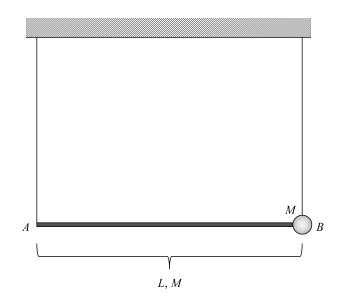
\includegraphics[width=0.55\textwidth]{imagenes/ayudantia_4_p4.png}
\end{center}

\vspace{0.2cm}
\textbf{Solucion}

\begin{enumerate}[a)]
\item \textbf{Centro de masa}
\[
x_{CM}=\frac{M\left(\frac{L}{2}\right)+M(L)}{2M}=\frac{3L}{4}.
\]

\item \textbf{Inercia total en el CM (Steiner)}

Primero, usando el extremo $A$ como referencia:
\[
I_{A}=\frac{ML^2}{12}+M\left(\frac{L}{2}\right)^2+ML^2
=\frac{4}{3}ML^2.
\]

Luego, con Steiner para llevar desde $A$ al centro de masa del sistema:
\[
I_{CM}=I_A-(2M)\left(\frac{3L}{4}\right)^2
=\frac{4}{3}ML^2-2M\frac{9L^2}{16}
=\frac{5}{24}ML^2.
\]

\item \textbf{Aceleración angular y tensión}

Sea $T$ la tensión izquierda y tomemos $y$ positivo hacia arriba.

Momento respecto al centro de masa del sistema:
\[
\sum \tau_{CM}:\quad -\frac{3L}{4}T=I_{CM}\alpha.
\]

Con $I_{CM}=\frac{5}{24}ML^2$:
\[
\alpha=-\frac{3LT}{4I_{CM}}. \qquad (1)
\]

Condición cinemática instantánea en $A$ (cuerda vertical e inextensible, con velocidad inicial nula):
\[
a_{Ay}=0 \;\Rightarrow\; a_{CMy}=\frac{3L}{4}\alpha. \qquad (2)
\]

Ecuación traslacional vertical del sistema total ($2M$):
\[
\sum F_y:\quad T-2Mg=2M a_{CMy}. \qquad (3)
\]

Usando (2) en (3):
\[
T-2Mg=2M\left(\frac{3L}{4}\alpha\right)=\frac{3}{2}ML\alpha. \qquad (4)
\]

Reemplazando (1) en (4):
\[
T-2Mg=\frac{3}{2}ML\left(-\frac{3LT}{4I_{CM}}\right)
=-\frac{9ML^2}{8I_{CM}}T.
\]

Con $I_{CM}=\frac{5}{24}ML^2$:
\[
T-2Mg=-\frac{27}{5}T
\quad\Rightarrow\quad
\frac{32}{5}T=2Mg
\quad\Rightarrow\quad
\boxed{T=\frac{5}{16}Mg}.
\]

Finalmente, usando (1):
\[
\alpha=\frac{9}{8}\frac{g}{L}
\]

Evaluación numérica:
\[
T=\frac{5}{16}(50.0)(9.81)=153.28\,\mathrm{N},
\]
\[
\alpha=\frac{9}{8}\frac{9.81}{2.50}=4.41\,\mathrm{rad/s^2}.
\]
\end{enumerate}
